%%=====================================================================================
%%
%%       Filename:  mm_figure_a.tex
%%
%%    Description:  
%%
%%        Version:  1.0
%%        Created:  Wednesday 10 January 2018
%%       Revision:  none
%%
%%         Author:  Dilawar Singh (), dilawars@ncbs.res.in
%%   Organization:  NCBS Bangalore
%%      Copyright:  Copyright (c) 2018, Dilawar Singh
%%
%%          Notes:  
%%
%%=====================================================================================
\RequirePackage{luatex85,shellesc}
\documentclass[crop,tikz]{standalone}
\usepackage{pgfplots}
\usetikzlibrary{calc,positioning}
\begin{document}
    \begin{tikzpicture}[scale=1, every node/.style={node distance=1mm} 
            , every label/.style={}
            , label position=north west
        ]
        \node[label={\bf a}] (panelA) {
            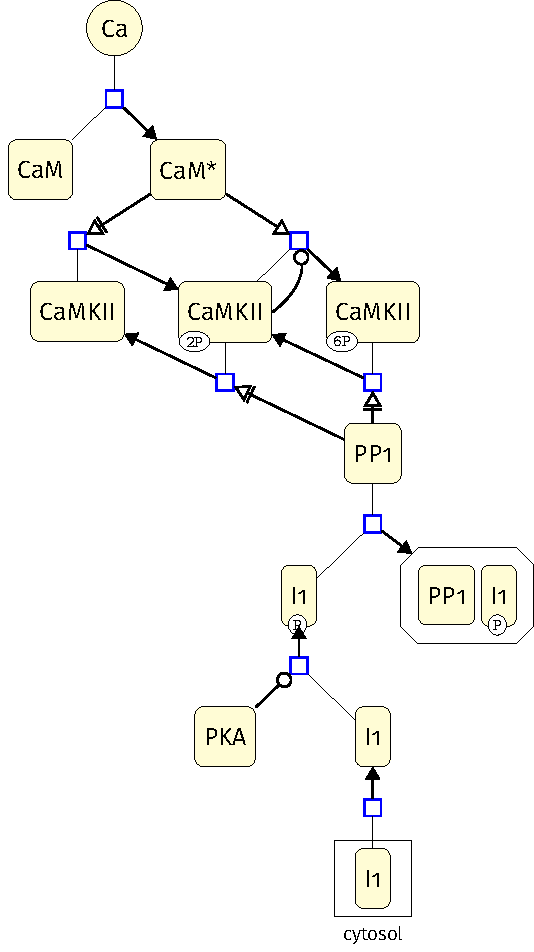
\includegraphics[width=0.3\textwidth]{./model_sbgn_pd_autolayout.pdf}
        };

        \node[right=of panelA,label={\bf b},xshift=5mm,yshift=20mm] (summary) {
            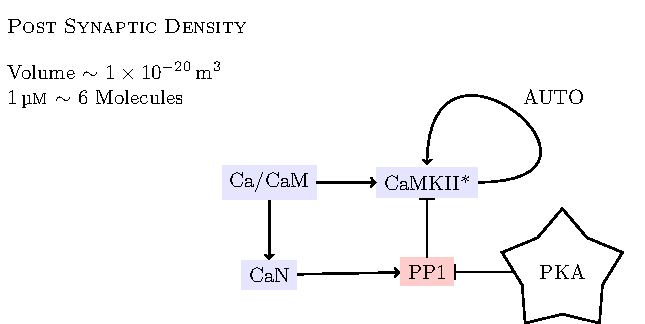
\includegraphics[width=0.45\textwidth]{./camkii_pp1_switch_summary.pdf};
        };

        \node[below=of summary,label={\bf c}] (slow_act) {
            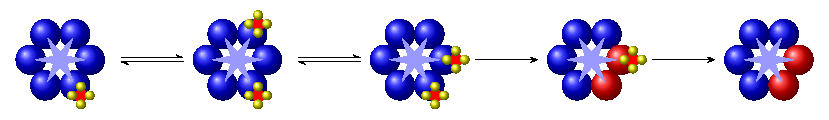
\includegraphics[width=0.45\textwidth]{./camk2_slow_activation.pdf}
        };

        \node[below=of slow_act,label={\bf d}] (fast_act) {
            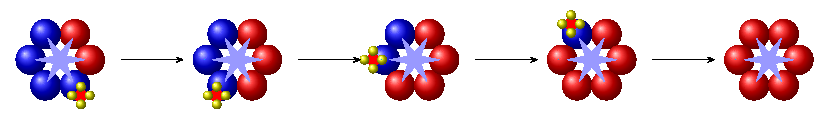
\includegraphics[width=0.45\textwidth]{./camk2_fast_activation.pdf}
        };

        \node[below=of fast_act,label={\bf e}] (subunit_exchange) {
            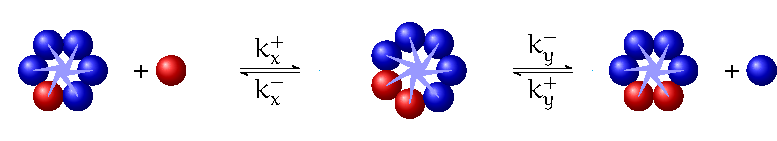
\includegraphics[width=0.45\textwidth]{./camkii_subunit_exchage.pdf}
        };
    \end{tikzpicture}    
\end{document}
